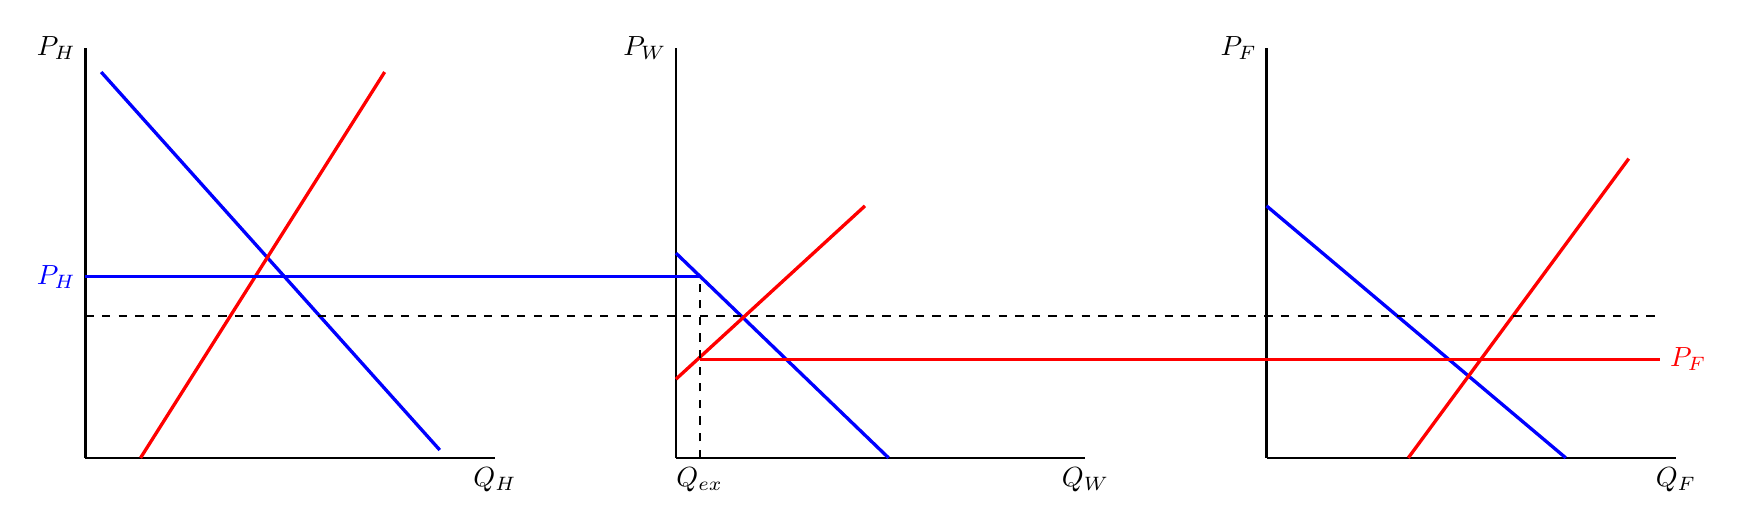
\begin{tikzpicture}[
    x=1cm,
    y=1cm,
    axis/.style={black, thick},
    demand/.style={blue, very thick},
    supply/.style={red, very thick},
    connection/.style={gray, thick, dashed}
]

% =========================================================
% PARAMETRI
% =========================================================

\def\axisheight{5.2}
\def\axiswidth{5.2}

% Posizione dei tre grafici
\def\xH{0}
\def\xW{7.5}
\def\xF{15}

% =========================================================
% MERCATO H
% =========================================================

% Assi
\draw[axis] (\xH,0) -- (\xH,\axisheight);
\draw[axis] (\xH,0) -- ++(\axiswidth,0);

% Etichette
\node[left]  at (\xH,\axisheight) {$P_H$};
\node[below] at ({\xH+\axiswidth},0) {$Q_H$};

% Domanda
\draw[demand]
({\xH+0.2},4.9) -- ({\xH+4.5},0.1);

% Offerta
\draw[supply]
({\xH+0.7},0) -- ({\xH+3.8},4.9);


% =========================================================
% MERCATO W
% =========================================================

% Assi
\draw[axis] (\xW,0) -- (\xW,\axisheight);
\draw[axis] (\xW,0) -- ++(\axiswidth,0);

% Etichette
\node[left]  at (\xW,\axisheight) {$P_W$};
\node[below] at ({\xW+\axiswidth},0) {$Q_W$};
\node[below] at ({\xW+0.3},0) {$Q_{ex}$};

% Domanda
\draw[demand]
(\xW,2.6) -- ({\xW+2.7},0);

% Offerta
\draw[supply]
(\xW,1.0) -- ({\xW+2.4},3.2);

% verticale
\draw[dashed, thick] ({\xW+0.3},0) -- ({\xW+0.3},2.3);

% =========================================================
% MERCATO F
% =========================================================

% Assi
\draw[axis] (\xF,0) -- (\xF,\axisheight);
\draw[axis] (\xF,0) -- ++(\axiswidth,0);

% Etichette
\node[left]  at (\xF,\axisheight) {$P_F$};
\node[below] at ({\xF+\axiswidth},0) {$Q_F$};

% Domanda
\draw[demand]
({\xF+0.0},3.2) -- ({\xF+3.8},0);

% Offerta
\draw[supply]
({\xF+1.8},0) -- ({\xF+4.6},3.8);


% =========================================================
% LINEE CHE COLLEGANO I MERCATI
% =========================================================

% Linea superiore: H -> W
%\draw[connection]
%({\xH+2.3},2.6) -- (\xW,2.6);

% Linea inferiore: W -> F
%\draw[connection]
%(\xW,1.0) -- ({\xF+2.6},1.0);

\draw[dashed, thick]
(\xH,1.8) -- ({\xF+5.0},1.8);

% =========================================================
% PREZZO COMUNE H-W
% =========================================================

\draw[blue, very thick]
(\xH,2.3) -- ({\xW+0.3},2.3);

\node[blue, left]
at (\xH,2.3) {$P_H$};


% =========================================================
% PREZZO COMUNE W-F
% =========================================================

\draw[red, very thick]
({\xW+0.3},1.25) -- ({\xF+5.0},1.25);

\node[red, right]
at ({\xF+5.0},1.25) {$P_F$};

\end{tikzpicture}
